%!TEX root = ../main.tex

%%%%%%%%%%%%%%%%%%%%%%%%%%%%%%%
%%%%%%%%%%%%%%%%%%%%%%%%%%%%%%%
\chapter{Methodical Modeling}
\label{chap:methodical-modeling}

\begin{textblock*}{.7\textwidth}(70mm-\offset,25mm-\offset)
        \begin{fquote}[Albert Einstein]
            All models are wrong, but some are useful.
        \end{fquote}
\end{textblock*}

This chapter mehodical modeling focusses on the description of thoughs and structures of the implementation in Python.
It is not evolving more than necessary details about the package {\itshape diffpssi}, but trying to comprehensible illustrate the structure of the algorithms theirselves and the necessaary bordering interfaces.

%%%%%%%%%%%%%%%%%%%%%%%%%%%%%%%
%%%%%%%%%%%%%%%%%%%%%%%%%%%%%%%
\section{Transformer Equipment Modeling}
\label{sec:transformer-modeling}

This section resp. focussed on the dynamics and model behavior of the transformer itself.
It is split according to the structure of the implementation itself, into the modeling of the $\Pi$-model and the tap changer control.
For the last mentioned, there are different control schemes implemented and thus described in the subsequent section.

%%%%%%%%%%%%%%%%%%%%%%%%%%%%%%%
\subsection{Implementing a $\Pi$-Representative Circuit with Variable Ratio}

Before detailing in the software side of the implemetation, some mathematical differences are explained.
This results on the one hand from the major differences in the standard literature, especially between \textcite{machowski_2020} and \textcite{kundur_2022}, resp. \textcite{milano_2010}.
On the other hand, these differences occur as well in the comparative and validation simulation software \textit{DIgSILENT PowerFactory}.
The use of these different models is described in its technical reference manual \quelle. 

\newpage
\subsubsection{Mathematical Description and Definitions}

\sidenote{Important definitions and literature differences}
Firstly it is important to comment on the use of indices in this thesis, and especially following for this chapter.
The index 1 is always referring to the \acs{LV} side, the index 2 to the \acs{HV} side. 
The impedances can be concentrated and related to either the \acs{LV}, or as usual to the \acs{HV} side of the transformer. 
The in \autoref{sec:trafo-model} used derivation is using a relation on the \acs{HV} side.
The same accounts for the definition of the \acs{OLTC} ratio $\underline{\vartheta}$.     
The \acs{OLTC} ratio $\underline{\vartheta}$ in this thesis is always placed on the HV side.
% If one wants to place this ratio on the \acs{LV} side, the in this thesis defined ratio has to be used reciprocal.
% For the simulation tool, this is crucial to understand and define correctly in order to acquire correct results.

\sidenote{Definition OLTC ratio}
This thesis focusses on an ideal tap changer model at first, other possible considerations from \autoref{sec:further-considerations} are neglected.
As vector groups are as well not considered, the tap ratio stays solely a rational number.
Like previously mentioned, and consequently described, the ratio $\vartheta$ is then pülaced on the \acs{HV} side of the transformer.
The \acs{OLTC} ratio $\vartheta$ is then defined as:
\begin{align}
        \vartheta_\mathrm{HV} &= 1 + k \cdot \Delta v \label{eq:tap-ratio-hv} \\[6pt]
        \text{with } k &\in [k_\mathrm{min};k_\mathrm{max}]; k_\mathrm{min} \equiv  -k_\mathrm{max} \label{eq:tap-pos}
\end{align}
Within this definition, $k_\mathrm{min}$ defines the minimum tap position, $k_\mathrm{max}$ the maximum \acs{OLTC} position. 
The variable $\Delta v$ defines the change of the ratio in percent for alterning one position.

% \sidenote{Representation of\\Vector Groups}
% Voltage angle shifting through the influence of vector groups, meaning a different wiring and thus magnetic coupling of the transformer can be expressed within the transformer model. 
% By mathematically applying a turning vector with the length of one to the overall tap ratio, this can be included in the model. 
% Mathematical, this is expressed by the following equation. 
% The characteristic number $n_\mathrm{T}$ is relating to to angle, with one step being equal to $30^\circ$ angle ratio.
% \begin{align}
%         \underline{a}_\mathrm{T} &= \exp(j \cdot n_\mathrm{T} \cdot \frac{\pi}{6}) \label{eq:vector-group}
% \end{align}

\subsubsection{Mathematical Different Representations}
\sidenote{Relation to the LV side}
When one either wants to relate the transformer admittance, or the tap ratio to the \acs{LV} side, a different admittance matrix definition has to be used.
The admittance matrix is then defined as:
\begin{align}
        \underline{\mab{Y}}_\mathrm{\Pi,T}&= 
        \begin{bmatrix}
            \underline{Y}_\mathrm{T} & -\underline{\vartheta}\underline{Y}_\mathrm{T} \\
            \underline{\vartheta}^*\underline{Y}_\mathrm{T} & -\underline{\vartheta}^*\underline{\vartheta}\underline{Y}_\mathrm{T}
        \end{bmatrix} \label{eq:admittance-oltc}
    \end{align}
The following mathematical result leads to a necessary change in the software implementation.
Either
\begin{itemize}
        \item the admittance matrix bus indices have to be changed,
        \item the tap ratio has to be reciprocal according to \autoref{eq:tap-ratio-lv}, or
        \item using the \acs{HV} side admittance matrix, but changing the tap ratio definition and the bus indices.
\end{itemize}
These different ways of variable and placing definitions also characterize the ways, the admittance matrix of the \acs{OLTC} transformer is derived from either \textcite{machowski_2020}, versus \textcite{kundur_2022}, \textcite{milano_2010}, or \textcite{burlakin_2024}.
Another thought or way of representing a transformer with off-nominal ratio is described in the appended \autoref{app:current-injection-model}.
\begin{align}
        \vartheta_\mathrm{LV} &= \frac{1}{1 + k \cdot \Delta v} \label{eq:tap-ratio-lv}
\end{align}

\subsubsection{Thoughts, Design, and Implemetation of Algorithmics}

\commenting{
        Base idea here: 
        \begin{itemize}[nosep]
                \item Show the thought process, design sketches and the implemetation algorithmics in the Python framework.
                \item Add a class diagram of the transformer model, with all needed interface / logable data, interface methods, and the abstract design.
                \item Describe addtional methods.
                \item Show the algorithmic implemetation logic of the Pi model, but not the Tap Changer, as this is seperated. 
        \end{itemize}
        Additionally interesting extensions:
        \begin{itemize}[nosep]
                \item How to automatically determine switching direction?\\
                -> switchin direction dependent on what? (load-flow direction?)
                \item Controller set points: also dependent on load flow?
                \item How can I change the transformer control setpoints to be load flow dependent?
                \item How can I ensure, utilization of the transformer is not $>S_\mathrm{n}$?
        \end{itemize}
}

%%%%%%%%%%%%%%%%%%%%%%%%%%%%%%%
\subsection{Tap Changer Control Modeling}

\commenting{This is the description of the ideas, development, and implementation of a OLTC control scheme.}

\subsubsection{Discrete Control Loop}
\commenting{
        \begin{itemize}[nosep]
                \item Describe implementation
                \item Describe benefits / drawbacks
                \item Control scheme
                \item Switching logic and behavior (voltage tracking)
        \end{itemize}
}

\sidenote{General aspects and references}
This control method represents the currently most used and thus representative control scheme for \acsp{OLTC}. 
With the mechanic nature of the switching mechanism, the control look can only access discrete ratios within time frames of around a few seconds. 
Such a discrete control loop is described by \textcite{milano_2011,milano_2010}. 
A scheme of this control loop is shown in \autoref{fig:discrete-control-loop}.

\begin{figure}[htb!]
        \centering
        \missingfigure{Discrete control loop}
        \caption{Discrete control loop of an \acs{OLTC}; scheme based on \textcite{milano_2011}}
        \label{fig:discrete-control-loop}
\end{figure}

This control loop type is beneficial due to its accurate representability of current \acs{OLTC} abilities. 
It gains access to assess stability within simulation environments, as analytical methods are not suited.

A negative aspect of a discrete control loop is the missing opportunity of generating a transfer function. 
This blocks the stability assessment with standard control engineering methods. 
Further, popular analysis methods like eigenvalue analysis is not possible, due to the lack of possibility to form derivatives.

% \lstinputlisting[caption={Output Function of the discrete OLTC controller},captionpos=b,style=style-python,label=lst:oltc-discrete]{images/code/oltc-discrete.py}

\sidenote{Implementation\\Structure}
\commenting{The structure of the implementation is illustrated in the block diagram of \autoref{fig:discrete-oltc-implementation}. 
The controller is actively chainging the algebraic funtions of the simulation environment, therefore it is quasi dynamic. 
The controller output logic is called, when updating the admittance matrix of the transformer. 
Additionally, the differential functions of the connected simple controllers, like integrators, PT1-blocks, etc., are called by the solver and are thus part of the differential equations. 
The logic determines the physical interpretation of the \acs{OLTC}, and therefore
\begin{enumerate}
        \item If the OLTC has to switch,
        \item When the switching operation is finished, and
        \item What the current, or in case after a switching the new, tap ratio is.
\end{enumerate}
It is important to note, that this structure relies on the calculation of the dynamic admittance matrix on each time step.}

\begin{figure}[htb!]
        \centering
        \missingfigure{Implementation structure of the discrete OLTC controller}
        \caption[Implementation structure of the discrete OLTC controller]{Implementation structure of the discrete OLTC controller}
        \label{fig:discrete-oltc-implementation}
\end{figure}

\sidenote{Output logic}
The output of the controller is based on the following logic.

\sidenote{Characterization plot and validation}

% \lstinputlisting[caption={Output Function of the discrete OLTC controller 2},captionpos=b,style=style-python,label=lst:oltc-discrete2]{images/code/oltc-discrete.py}

\subsubsection{Continous Control Loop}

\begin{figure}[htb!]
        \centering
        \includegraphics[width=.7\linewidth]{development_files/validation/data/oltc_control_characterization.pdf}
        \caption[Characterization of the OLTC control loops]{Characterization of the OLTC control loop; the input function simulates the to be regulated voltage, the output functions are characterized by $o(t)=i(t) \cdot \underline{\vartheta}_\mathrm{trafo}$}
        \label{fig:oltc-control-characterization}
\end{figure}

\subsubsection{Control Schemes for the Fast Switching module}
\commenting{
        \begin{itemize}[nosep]
                \item Describe implementation
                \item Describe benefits / drawbacks
                \item Control scheme
                \item Switching logic and behavior (voltage tracking)
        \end{itemize}
}
\sidenote{Functional basics of a \acs{FSM}}
Describe the operational logic and structure of the \acf{FSM} first.

\sidenote{Control logic}
A control logic for a so called \acs{FSM} has been presented from \textcite{burlakin_2024}, and illustrated in \autoref{fig:fsm-control-loop}.

\begin{figure}[htb!]
        \centering
        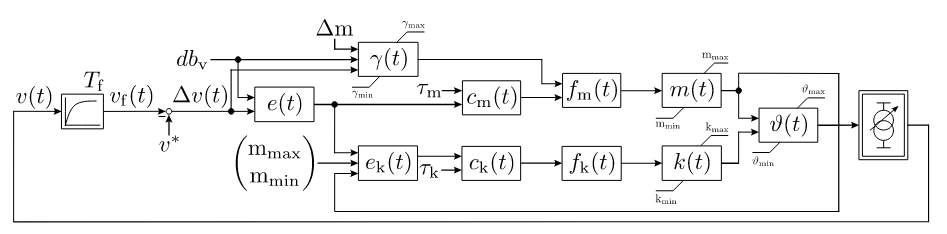
\includegraphics[width=\textwidth]{modeling/fsm_control_scheme.png}
        \caption[Control loop of a \acf{FSM}]{Control loop of a \acs{FSM}; scheme based on \textcite{burlakin_2024}}
        \label{fig:fsm-control-loop}
\end{figure}

\sidenote{Implementation\\differences}
However, the implementation logic in Python is slightly differing from the presented scheme in \autocite{burlakin_2024}, simply for not overcomplication of the code and therefeore debugging. 
The implementation is similar to the afore discussed one of a standard \acs{OLTC} controller. 

\sidenote{Characterization and validation}

%%%%%%%%%%%%%%%%%%%%%%%%%%%%%%%
\subsection{Experimental: Extended Ideas and Improvements}

\subsubsection{Operational Oriented FSM Control}

\subsubsection{Alternative Tap Skipping Logic}

\subsubsection{Varying the Voltage Setpoint and Target Calculation}

\commenting{
        Here, another idea of control target creation shall be mentioned. 
        Instead of a fixed bus voltage reference, the difference of both bus voltages is considered. 
        Further, the sign of that difference is used to determine the direction of the tap change.
}

% %%%%%%%%%%%%%%%%%%%%%%%%%%%%%%%
% %%%%%%%%%%%%%%%%%%%%%%%%%%%%%%%
% \section{Supplementary Modeling and Advancements}

% As the python framework is currently missing some representations of components, this chapter aims to describe the implementation of those. Mainly focussing on source and load models, as the later considered test, benchmark, and use case networks require alternative behaviors. 

% %%%%%%%%%%%%%%%%%%%%%%%%%%%%%%%
% \subsection{ZIP Load Model}

% \commenting{Why important?}

% Mostly, a polynomial load model is used. It is called ZIP-model, as there are individual contributions to constant impedance $\underline{Z}$, constant current $\underline{I}$, and constant power $P$, or respectively $Q$, are considered. The model is described by \textcite{IEEELoad_2022}. Either two ways of mathematical description are considered valid, dependent on the allowed influence of the frequency deviation. The use of periodized phasor representation, typical for a \acs{RMS} simulation, is missing or often neglecting this frequency information. Therefore the set of \autoref{eq:zip-1} and \autoref{eq:zip-2} is considered sufficient and implemented in the Python framework.
% \begin{align}
%         P&=P_n \cdot \Bigg[ p_1 \Bigg(\frac{U}{U_n}\Bigg)^2 + p_2 \Bigg(\frac{U}{U_n}\Bigg) + p_3 \Bigg] \label{eq:zip-1} \\[12pt]
%         Q&=Q_n \cdot \Bigg[ q_1 \Bigg(\frac{U}{U_n}\Bigg)^2 + q_2 \Bigg(\frac{U}{U_n}\Bigg) + q_3 \Bigg] \label{eq:zip-2} \\[12pt]
%         \text{with} \quad &p_i \in [0,1] \quad \text{and} \quad q_i \in [0,1] \notag
% \end{align}

% \commenting{Characteristics?}

% \begin{figure}[htb!]
%         \centering
%         \includegraphics[width=\linewidth]{development_files/data/zip-load_characterization_full.pdf}
%         \caption[Characterization of the ZIP load model]{Characterization of the ZIP load model; with (upper) the result of the impedances dependent on the voltage at the connected bus, and (lower) the resulting power consumption of the different models, representative only the real power $P$}
%         \label{fig:zip-charac}
% \end{figure}

% \commenting{How does it look like in the simulation environment?}

% \begin{align}
%         P&=P_n \cdot \Bigg[ p_1 \Bigg(\frac{U}{U_n}\Bigg)^2 + p_2 \Bigg(\frac{U}{U_n}\Bigg) + p_3 \Bigg] \cdot (1+k_{pf} \Delta f) \label{eq:zip-with-f-1} \\[12pt]
%         Q&=Q_n \cdot \Bigg[ q_1 \Bigg(\frac{U}{U_n}\Bigg)^2 + q_2 \Bigg(\frac{U}{U_n}\Bigg) + q_3 \Bigg] \cdot (1+k_{qf} \Delta f) \label{eq:zip-with-f-2} \\[12pt]
%         \text{with} \quad &\sum_{i=1}^{3} p_i =1 \quad \text{and} \quad \sum_{i=1}^{3} q_i =1 \notag
% \end{align}

% Although the subset of \autoref{eq:zip-with-f-1} and \autoref{eq:zip-with-f-2} would consider a relation to the frequency at the given time, it is not used. The use of periodized phasor representation, typical for a \acs{RMS} simulation, is missing this information in the framework diffpssi. Therefore the set of \autoref{eq:zip-1} and \autoref{eq:zip-2} is implemented in the Python framework. It has to be mentioned, because the comparison tool PowerFactory is using this load model, though in some parts of the simulation results are showing a slightly bigger error.

% %%%%%%%%%%%%%%%%%%%%%%%%%%%%%%%
% \subsection{Induction Machine Models}

% As one of the most important loads to consider, especially for many load driven instability mechanisms, the \ac{IM} is a crucial component, \quelle

% \commenting{
%         Just briefly:
%         \begin{itemize}[nosep]
%                 \item Why is it crucial?
%                 \item How do the instability mechanisms work and look like?
%                 \item What are the different types of \acsp{IM} modeling (complete and dynamic, static, \dots)
%         \end{itemize}
% }

% Three main ways of \acs{IM} modeling are relevant to mention in this section:
% \begin{enumerate}
%         \item Static model as introduced in \textcite{IEEELoad_2022},
%         \item a dynamic 'fixed-speed' \acs{IM} model, and
%         \item a doubly fed \acs{IM} model.
% \end{enumerate} 
% The last ones are mentioned and further described in \textcite{machowski_2020}. Least model requires very detailed information, and shall be suitable for \acs{SMIB} models for machine behavior studies or similar. The second model is suitable for network analysis and machine behaviors. The first model applies for high perception of \acsp{IM} in total loading of the network. As referencing to \textcite{IEEELoad_2022}, is is similar implemented as the before mentioned ZIP load model, considering characteristic equations for its real power $P$ and reactive power $Q$. Both models shall be described in the following section.

% \subsubsection{Static Model of Induction Machines}

% For this operational unit type is a detailed dynamic modeling possible. With some considerations, it can be sufficient, modeling this equipment just with the  The model is described by \textcite{IEEELoad_2022} as formulated in following set of equations. %\autoref{eq:im-model}.

% \begin{align}
%         P&=\Bigg( R_\mathrm{s} + \frac{R_\mathrm{r}}{s} \Bigg) \cdot \frac{U^2}{\Big( R_\mathrm{s} + \frac{R_\mathrm{r}}{S} \Big)^2 + (X_\mathrm{\gamma s} + X_\mathrm{\gamma r})^2} \\[12pt]
%         Q&=(X_\mathrm{\gamma s} + X_\mathrm{\gamma r}) \cdot \frac{U^2}{\Big( R_\mathrm{s} + \frac{R_\mathrm{r}}{S} \Big)^2 + (X_\mathrm{\gamma s} + X_\mathrm{\gamma r})^2} + \frac{U^2}{X_\mathrm{s}}
% \end{align}
% \mycomment[MK]{Is here really a difference between the two s in the equations?}

% \commenting{Briefly describe the implementation.}

% \subsubsection{Dynamic 'fixed-speed' Induction Machine model'}

% \ai{\textbf{From ChatGPT:}

% The dynamic model of \acsp{IM} is essential for accurately representing their behavior under various operating conditions. This model includes the differential equations that describe the machine's electrical and mechanical dynamics. The equations are typically derived from the machine's equivalent circuit and can be expressed in the d-q reference frame.

% The dynamic model can be represented by the following set of equations:

% \begin{align}
%         \frac{\dd\psi_\mathrm{d}}{dt} &= v_\mathrm{d} - R_\mathrm{s} i_\mathrm{d} + \omega \psi_\mathrm{q} \\[12pt]
%         \frac{\dd\psi_\mathrm{q}}{dt} &= v_\mathrm{q} - R_\mathrm{s} i_\mathrm{q} - \omega \psi_\mathrm{d} \\[12pt]
%         \frac{\dd\omega}{dt} &= \frac{1}{J} (T_m - T_e - B \omega)
% \end{align}

% where:
% \begin{itemize}
%         \item $\psi_\mathrm{d}, \psi_\mathrm{q}$ are the d-q axis flux linkages
%         \item $v_\mathrm{d}, v_\mathrm{q}$ are the d-q axis voltages
%         \item $i_\mathrm{d}, i_\mathrm{q}$ are the d-q axis currents
%         \item $R_\mathrm{s}$ is the stator resistance
%         \item $\omega$ is the rotor angular velocity
%         \item $T_\mathrm{m}$ is the mechanical torque
%         \item $T_\mathrm{e}$ is the electromagnetic torque
%         \item $J$ is the moment of inertia
%         \item $B$ is the damping coefficient
% \end{itemize}

% The electromagnetic torque $T_e$ can be calculated as:

% \begin{align}
%         T_e = \frac{3}{2} p (\psi_d i_q - \psi_q i_d)
% \end{align}

% where $p$ is the number of pole pairs.

% This dynamic model allows for the simulation of the \acsp{IM} transient response to changes in voltage, frequency, and load conditions. It is particularly useful for studying stability and control strategies in power systems.

% }

% \commenting{Briefly describe the implementation.}

% % \subsection{PQ Source without Machine Dynamics}

% % \todo[inline]{Necessary? Because one can use just an inverter at defined operation points}

% % \commenting{Isn't that quite the same as the ZIP load model, but with inversed Power characteristics? Or is there more, for example when looking at a short circuit event\dots}

% % \commenting{
% %         These sections (per module / model) should contain roughly follwing information and / or structure:
% %         \begin{enumerate}
% %                 \item Why is this model important?
% %                 \item How is it implemented?
% %                 \item What are the characteristics (show in plots, description, etc.)?
% %                 \item How does it look like in the simulation environment? -> Smaller example networks, like the \acs{SMIB} model; most likely combined with verification data of PowerFactory.
% %         \end{enumerate}
% % }


%%%%%%%%%%%%%%%%%%%%%%%%%%%%%%%
%%%%%%%%%%%%%%%%%%%%%%%%%%%%%%%
\section{Application of Voltage Stability}
\label{sec:application-voltage-stability}

% \commenting{
%         General though process:
%         \begin{itemize}[nosep]
%                 \item Which indices can be implemented?
%                 \item Which make sense? (Aspects: Calculation time, accuracy, accessability: e.g. also for using PowerFactory Data)
%                 \item Implementation of a framework:\\
%                 -> Capable of using diffpssi or PF data, calculation of time series indices, EAC for voltage angle stability on machines, ... \\
%                 -> Output characteristics: Voltage stability indices over time, critical time point of voltage stability, critical time point of voltage angle stability on machines...
%         \end{itemize}
%         Further nice to have / additional:
%         \begin{itemize}[nosep]
%                 \item Index combination and \glqq traffic light\grqq\~monitoring
%                 \item Local mapping
%                 \item Weak point identification
%         \end{itemize}
% }

\subsection{Generation of Nose Curves}
\label{sec:nose-curves}

This section describes the implementation of a prevoiusly discussed static voltage analysis tool.
The generation of nose curves helps in finding the critical loading of the system at the bus of interest, although it is static nature. 

\subsubsection{Basic Simplification Idea}

\textcite{ajjarapu_1992, ajjarapu_2007} are presenting a method for numerical calculation of nose curves in their work. 
It is called {\itshape Continuation Power Flow} and is based on a modified Newton-Raphson method.
The differences rely in a slightly different definition of the power flow equations, considering a load factor $\lambda$.
Combined with a predictor-corrector iterative solver method, this algorithm is capable of nose curve calulation, and finding the critical loading of the system.
While in the first work \autocite{ajjarapu_1992}, only the upper part of the curve including the critical point is calculated, the second work \autocite{ajjarapu_2007} is capable of calculating the complete curve with both solutions. 
As the trade off between implementation effort and the benefits, this method is not exchanging the reduced and simplyfied one.

While this method would be appealing to implement, an additional load flow algorithm, solver, and wrapper seem not profitable for this thesis.
An idea was occuring, just iteratively using the available implemented standard Newton-Raphson algorithm, and implementing a wrapper around it.
The proposed result should be the upper and stable nose curve branch, with the critical point of active power loading.
This shall seem sufficient, as the lower branch solutions are not stable load flow solutions.

The often used parameterization of a function of voltage dependent on the active power and the power angle $\phi$ should be implemented.
In mathematical term, this is expressed as \autoref{eq:pv-mathematical}.
\begin{align}
        \vert \underline{V} \vert : P &\mapsto f(P, \phi) \label{eq:pv-mathematical} \\[6pt]
        Q : \underline{V} &\mapsto f(\underline{V}, \phi) \label{eq:vq-mathematical}
\end{align}
Under consideration of a complex representation of voltage and powers, this algorithm can calculate $V-Q$ curves as well. 
Mathematically this is expressable as \autoref{eq:vq-mathematical}.

\subsubsection{Implementation Details}

% \commenting{
%         Basic idea:
%         \begin{itemize}
%                 \item Generic utilization of the PSS class for iterative load flow calculation
%                 \item Saving the results in a re-callable attribute
%                 \item Added automized plotting function
%                 \item Show class diagram and interfaces
%         \end{itemize}
% }

\begin{wrapfigure}[12]{r}{0.4\textwidth}
        % \vspace{-20pt}
        \centering
        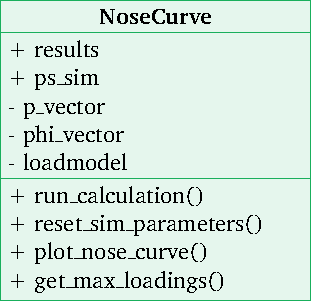
\includegraphics[width=.9\linewidth]{tikz_graphics/images/class_diagram_nosecurve_red.pdf}
        \caption{Class diagram of the NoseCurve class in the package diffpssi}
        \label{fig:nose-curve-characterization}
\end{wrapfigure}
The implementation of the nose curve generation is realized as a class in the package {\itshape diffpssi.stability$\_$lib.voltage}.
Its class diagram with all attributes and methods is shown in \autoref{fig:nose-curve-characterization}, an extended version is included in \autoref{app:nose-curve}.
For an easy and generic use of the {\itshape diffpssi} package, {\itshape PowerSystemSimulation} objects are used, as well as the function {\itshape do$\_$load$\_$flow()} from the package.

As the afore mentioned idea, the method for running the calculation is a iterative wrapper of the load flow calculation. 
This can be as well applied for mutiple busses as a list input.
At first, the grid and therefore models of the {\itshape PowerSystemSimulation} object has to be cleared with the method {\itshape reset$\_$sim$\_$parameters()}.
Then the active power vector is iterated as load input, together with the power angle $\phi$ for the reactive power in the model.
Important to note here, is the usage of an {\itshape **kwargs} argument.
The callable for the model is called with load parameters for each load bus as the Bus name, and a list with active and reactive power.
The initials of this grid callable are used as the standard values, so only one bus can be varied at a time.
The result is saved as a {\itshape pandas DataFrame} in a dict, with the keys being the bus names.

The method {\itshape plot$\_$nose$\_$curve()} is used to plot the results, and is using the {\itshape matplotlib} package.
Further, the method {\itshape get$\_$max$\_$loadings()} can provide details about the critical point.
Giving back a dict with keys as bus names, the values itself are dicts with key of the power angle parameter $\tan \phi$ and the values as {\itshape pandas DataFrame}.
The contained details are maximum active power $P_\mathrm{max}$, the reactive power $Q$ at this point, and the voltage magnitude $\vert \underline{V} \vert$ at the bus.

\subsubsection{Results of the Nose Curve Generation}

The following figure \autoref{fig:nose-curve-simple-grid} shows the generated nose curve for a simple grid as illustrated in \autoref{fig:single-line-voltage-stability}.
The grid is characterized at Bus 1, with a varying power angle as parameter $\tan \phi$.
The power angle $\tan \phi$ is used to vary the power factor of the load, thus representing different load characteristics, as
\begin{align}
        \tan \phi &= \frac{Q}{P}. \notag %\label{eq:tan-phi} \\[6pt]
\end{align}
Displayed are a few combinations with different load characteristics, leading to a different possible maximum acitve power transfer.
\autoref{fig:nose-curve-simple-comp} shows the comparison between the analytical calculation and the implemented solution.
The analytical calculation is carryied out with the method described in \autoref{sec:analytical-voltage-stability}.
For this specific example, the complete calculation, including the set of used parameters, is shown in \autoref{app:analytical-nose-curve}.
What seems conspicious is the missing lower part of the curve, meaning the second possible solution when solving the power flow equations.
Although this seems like a major drawback, the resulting curve contains all the necessary parts, where a stable solution can occur. \quelle
The solution is reaching exactly until the critical point of power transfer.

\begin{figure}[htbp!]
        \centering
        \includegraphics[width=\linewidth]{development_files/theoretical/plots/simple_load_B1_nose_curve.pdf}
        \caption[Examplary generated nose curve for a simple generator - load grid]{Examplary generated nose curve for a simple generator - load grid for various power angle level parameters $\tan \phi$; Applied on the grid of \autoref{fig:single-line-voltage-stability} with a characterization at Bus 1}
        \label{fig:nose-curve-simple-grid}
\end{figure}

\begin{figure}[htbp!]
        \centering
        \includegraphics[width=\linewidth]{development_files/theoretical/plots/simple_load_B1_nose_curve_w-theoretical.pdf}
        \caption[Comparison between the analytical calculation and the implemented solution]{Comparison between the analytical calculation and the implemented solution}
        \label{fig:nose-curve-simple-comp}
\end{figure}



%%%%%%%%%%%%%%%%%%%%%%%%%%%%%%%
%%%%%%%%%%%%%%%%%%%%%%%%%%%%%%%
\section{Summary in Short and Simple Terms}